\section{Introduction and motivation}

In \cite{arxiv:meta-metta-opsem:meredith} we described a register
machine based operational semantics for $\mathsf{MeTTa}$. While this
has some utility for proving the correctness of compilers, it is not
conducive for reasoning about types and other more abstract aspects of
$\mathsf{MeTTa}$-based computation. Here we present a calculus,
together with a efficient implementation and prove the correctness of
the implementation.

Additionally, we use the $\mathsf{OSLF}$ algorithm developed by
Meredith, Stay, and Williams to calculate a spatial-behavioral type
system for $\mathsf{MeTTa}$. Further, we adapt a well known procedure
for proving the termination of rewrites to provide a token-based
security model for the calculus and implementation. Beyond that we
derive versions of fuzzy, stochastic, and quantum execution modes,
automatically.

\begin{figure}
  \centering
  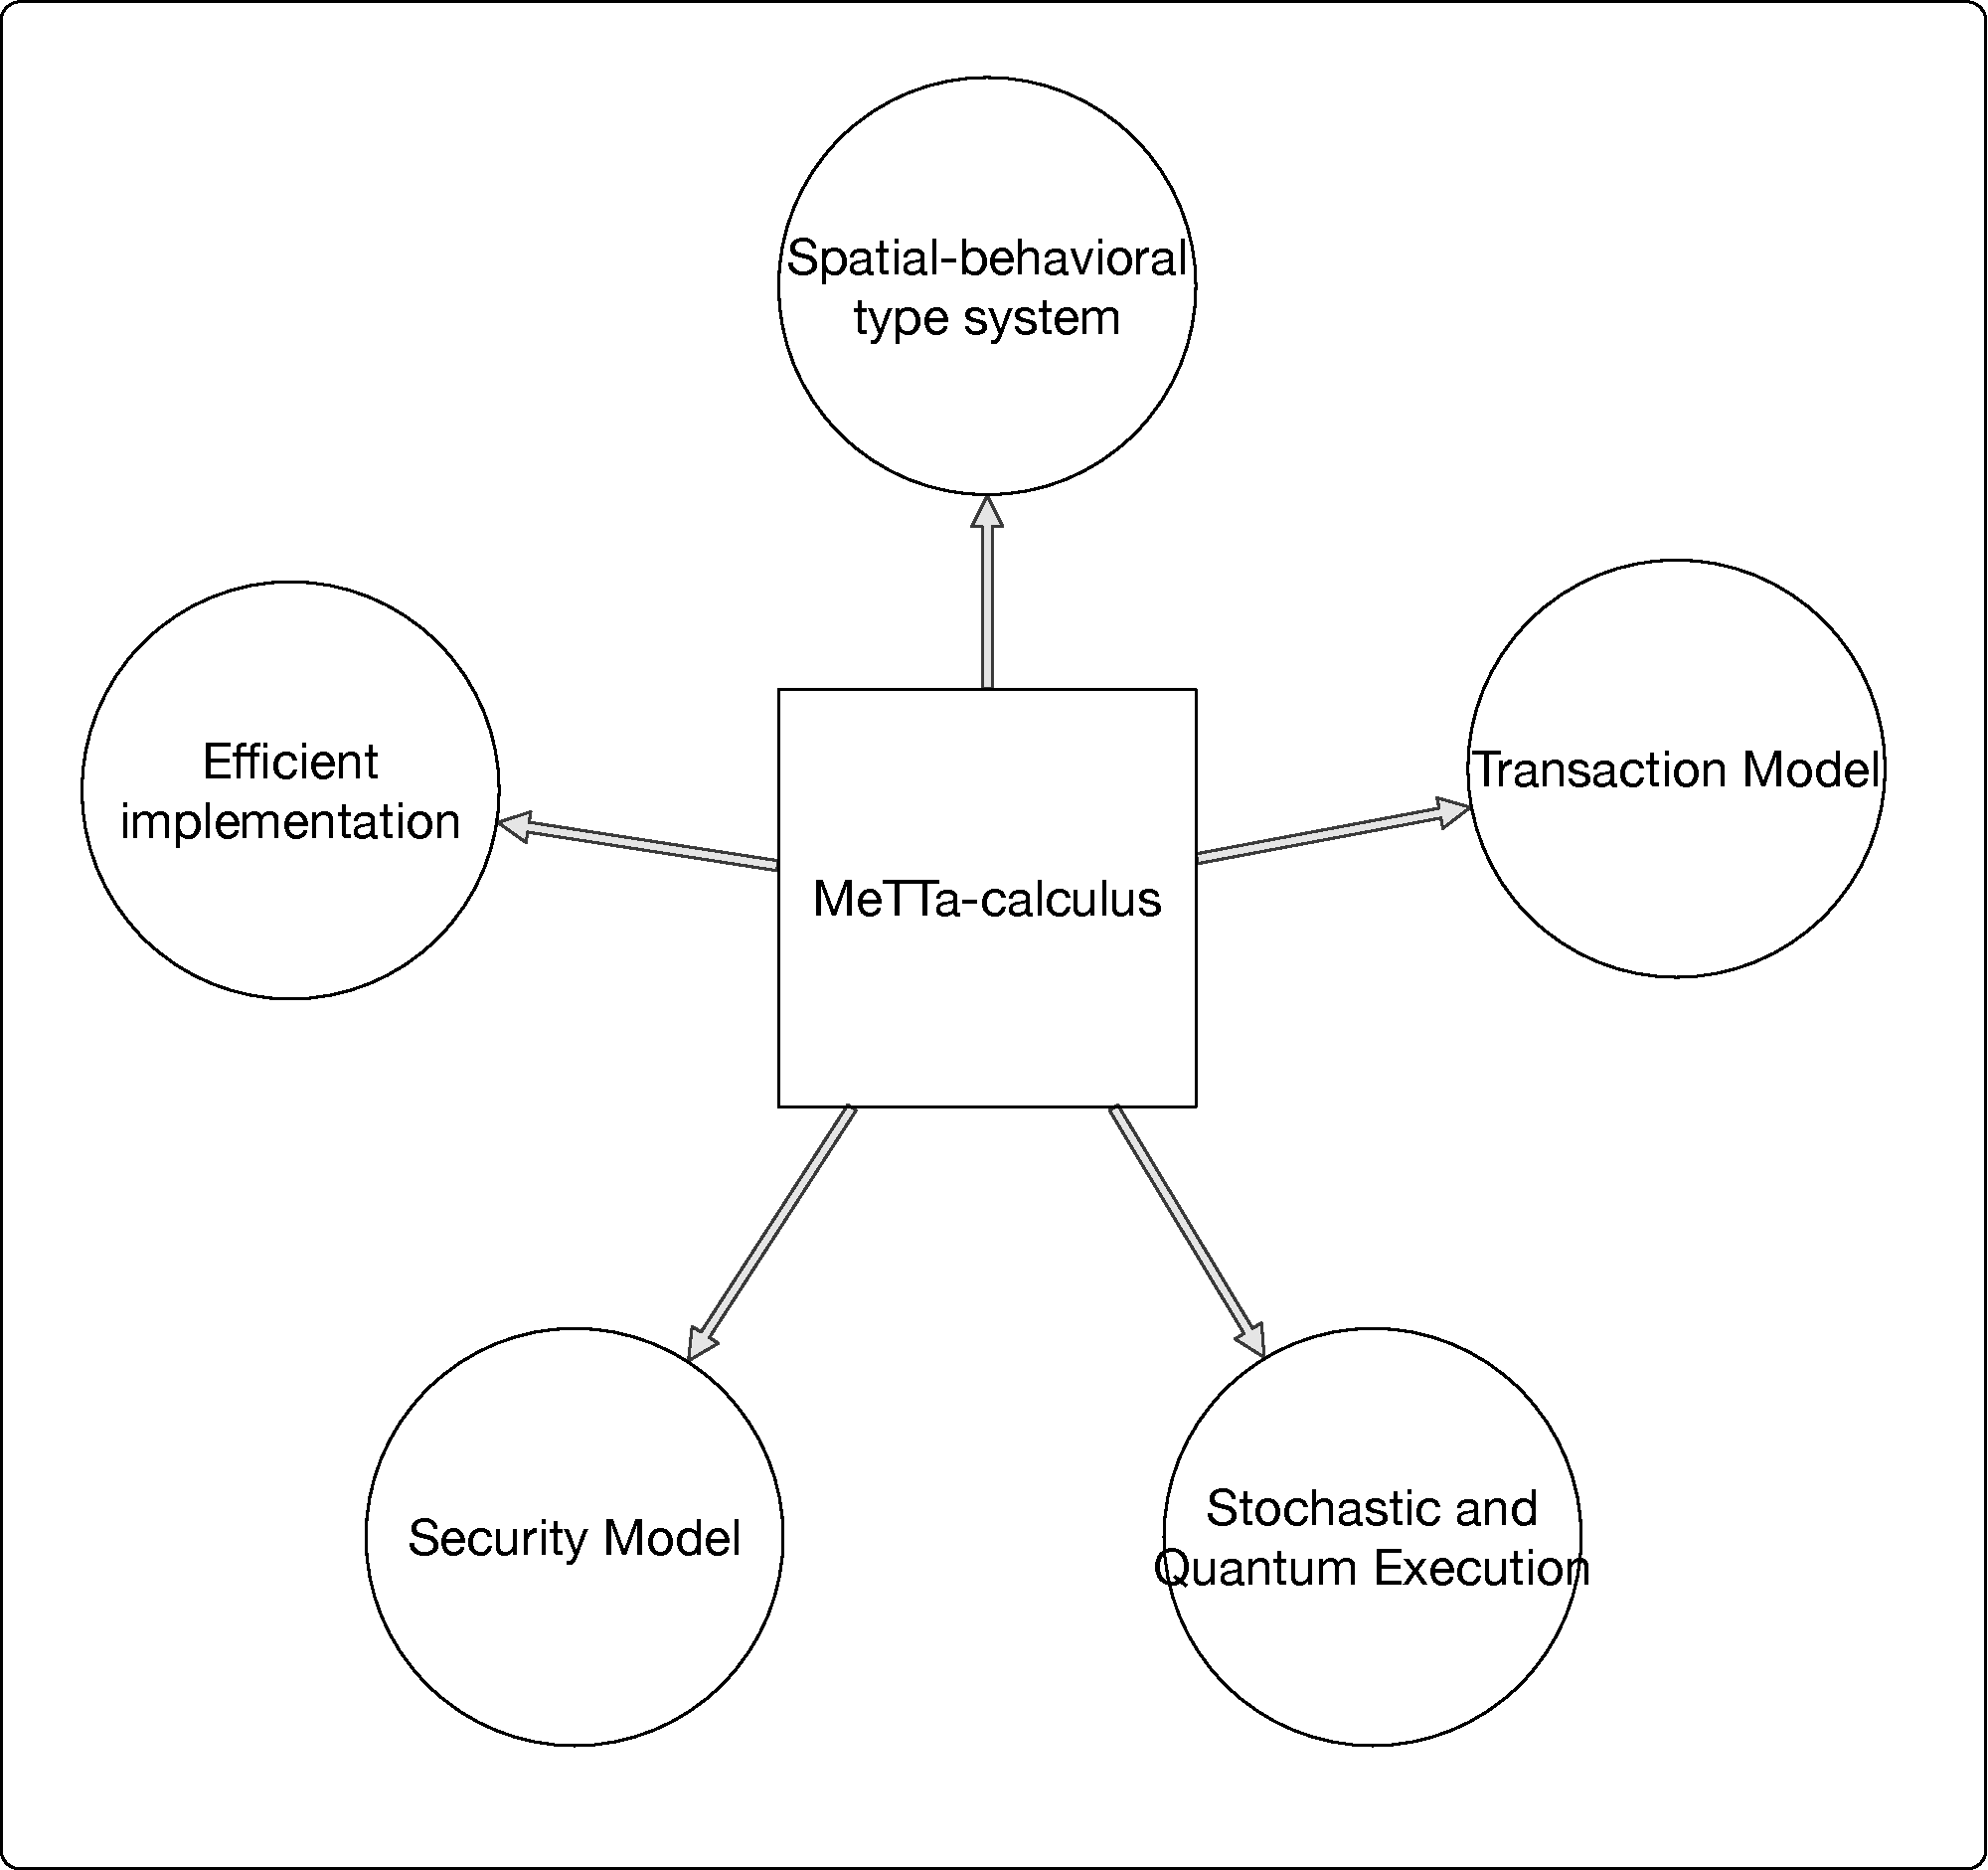
\includegraphics[scale=0.25]{MeTTaCalculusGenerationOfFeatures.pdf} \\
  \caption{Generating features from the $\mathsf{MeTTa}$-calculus}
\end{figure}

In general, presenting $\mathsf{MeTTa}$ as a graph structured lambda
theory, otherwise known as a structured operational semantics, not
only has the benefit that implementation follows the
correct-by-construction methodology, but may be used to automatically
derive and extend $\mathsf{MeTTa}$ with much needed features for
programming real applications in a distributed and decentralized
setting, as well as supporting well established programming paradigms,
such as semi-colon delimited sequential assignment programs.
